
\appendix

\appendices




\subsection{Threat Model}
 An organization offers several siloed LLM services, each compartmentalized with distinct stacks and compliance boundaries. An adversary interacts with these services via standard prompt interfaces (Figure~\ref{fig:system-architecture}). The adversary has no access to internal artifacts (such as logs, fingerprints, or defense details) and cannot tamper with compliance boundaries. The adversary sends prompt-injection attack variants to exploit vulnerabilities across these services. In \tool, if a prompt injection attack is detected in one of these services, the goal is to share this threat intelligence with other peer services while preserving privacy. \tool shares a privacy-preserving fingerprint of the detected attack, which peer services can correlate in a privacy-preserving manner, thereby improving organization-wide visibility of attacks.

\subsection{Motivating Example}
The motivation in context of compliance boundaries is discussed in earlier sections (Section~\ref{sec:introduction} and Section~\ref{sec:design}). Here is another motivating example to demonstrate \tool effectiveness. 
Consider a cloud provider offering generative AI services to multiple independent enterprise customers, hereafter referred to as Company A and Company B. Note in this scenario companies are customers of the cloud provider. Due to strict regulatory requirements and contractual obligations, these two customers operate in completely separate compliance boundaries. Their data cannot be shared, and their logging systems are entirely siloed.
 
Now suppose a malicious actor launches prompt injection attacks against both companies' AI services. Because the data between Company A and Company B cannot be correlated or shared directly, each company's security team operates in isolation. They may detect anomalies independently, but they have no way to identify that the same attacker is targeting both services, nor can they assess the full scale and sophistication of the attack campaign.
 
This is where \tool provides value. By generating privacy-preserving fingerprints of detected malicious prompts, \tool enables the cloud provider to correlate threat intelligence across these two isolated compliance boundaries without exposing the original prompts or violating privacy regulations.


 \begin{table}[h]
\centering
\caption{Performance comparison on the WildJailbreak dataset.}
\label{tab:wildjailbreak}
\begin{tabular}{lccc}
\hline
Metric & Dense (No Privacy) & \tool & Gap \\
\hline
Accuracy@1 & 99.25\% & 93.82\% & 5.43\% \\
Accuracy@2 & 99.70\% & 97.54\% & 2.16\% \\
Accuracy@3 & 99.70\% & 98.54\% & 1.16\% \\
Accuracy@5 & 99.90\% & 99.3\% & 0.6\% \\
\hline
\end{tabular}
\end{table}


\begin{figure}
    \centering
    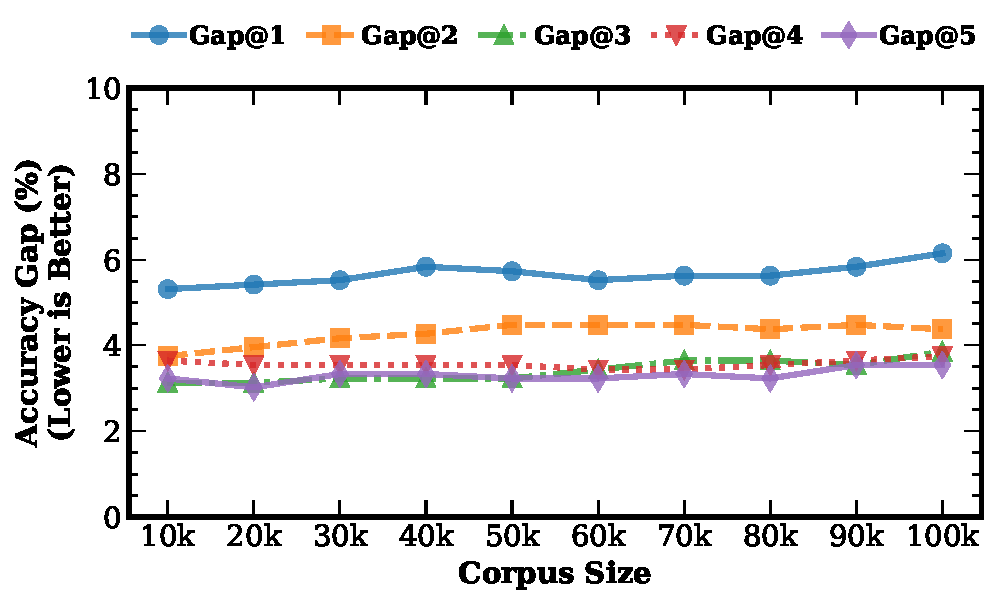
\includegraphics[width=\linewidth]{exp_results/real-world-scenario-results/accuracy_gap_lines_all_k.pdf}
    \caption{Accuracy@k gap (Dense Embeddings - \tool) across corpus sizes.  Rapid narrowing for higher k demonstrate that binary quantization plus local DP introduce a constant, not compounding, utility cost.}
    \label{fig:hybrid-accuracy-gap}
\end{figure}



\begin{figure}[t]
        \centering
        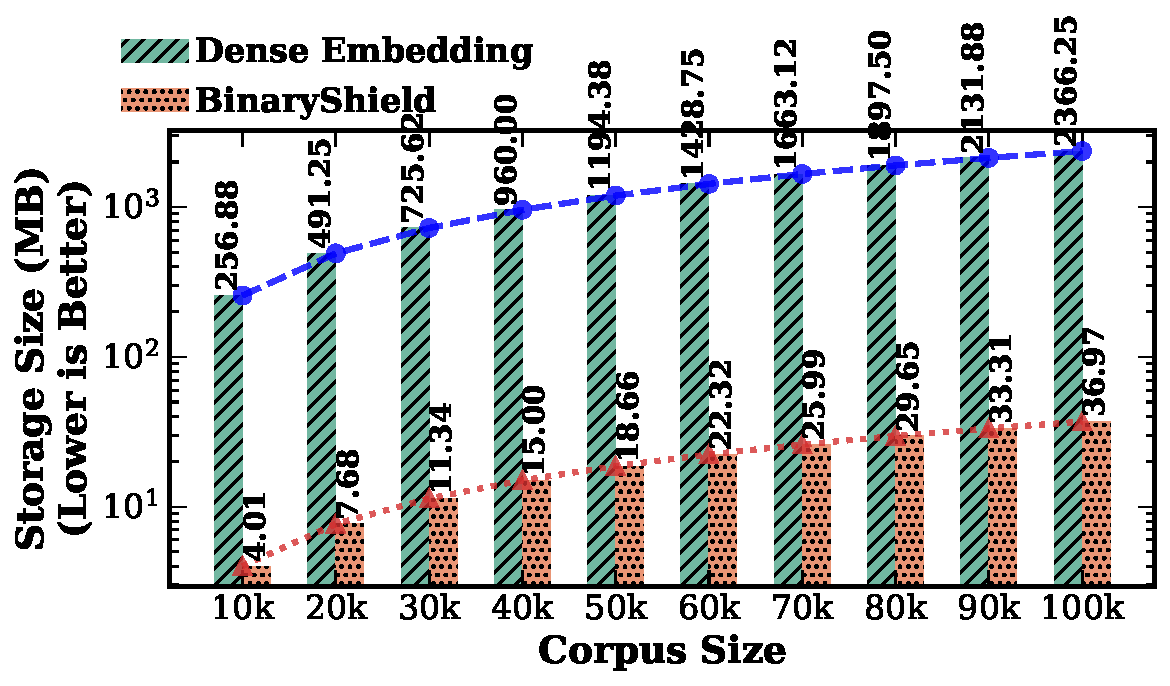
\includegraphics[width=\linewidth]{exp_results/real-world-scenario-results/storage_size_scalability_hybrid.pdf}
        \caption{Storage size comparison demonstrating \tool's 64x reduction compared to dense embeddings. Dense embeddings scale from 256.88 MB at 10K entries to 2,366.25 MB at 100K entries, while \tool requires only 4.01 MB to 36.97 MB respectively, enabling cost-effective long-term threat intelligence retention.}
        \label{fig:storage-size-comparison}
    
\end{figure} 



\begin{lstlisting}[style=customprompt, basicstyle=\ttfamily\scriptsize,caption={Template for generating adversarial prompt variants via lexical substitution.}, label={prompt:words-flipped}]
Understand this adversarial prompt: <original prompt>. Now generate synonyms for the following words: <words to change>. Return the JSON with the field `words_changes_to` containing the synonyms in order.
\end{lstlisting}


\begin{lstlisting}[style=customprompt, basicstyle=\ttfamily\scriptsize,caption={Template for generating adversarial prompt variants via full-sentence paraphrasing.}, label={prompt:paraphrase}]
Paraphrase the following adversarial prompt while maintaining the attack intent and purpose. Original prompt: <original prompt>. Return the JSON with the field `generated_response`.
\end{lstlisting}

\subsection{Synthetic Variant Attack Potency and Evaluation on WildJailbreak Dataset}
We conduct an evaluation to test the attack potency of our synthetic variants, specifically examining whether they maintain attack potency comparable to original attacks. We conduct a study comparing 500 original attack prompts~\cite{shen2024doanything} and their synthetic variants (V\_Paraphrase) using GPT-4.1-nano combined with Azure's Prompt Shields for attack detection in an enterprise setting. Original attacks achieve an 80.4\%  detection rate, while synthetic variants achieve a 78.0\%. These near-identical detection rates demonstrate that the synthetic variants preserve adversarial characteristics comparable to the original attacks.


Several jailbreak datasets exist~\cite{WildJailbreak, shen2024doanything, luo2024jailbreakv, JailbreaksOverTime}. We evaluate \tool on~\cite{shen2024doanything} in Section~III and on WildJailbreak~\cite{WildJailbreak} here similar to Section~III-C. Table~\ref{tab:wildjailbreak} confirms \tool's robustness on WildJailbreak. It achieves 93.82\% Accuracy@1 on a 100K corpus of benign and adversarial prompts, retaining 94.5\% of the non-private baseline, consistent with our earlier results (Figures~\ref{fig:hybrid-accuracy-scalability} \&~\ref{fig:hybrid-accuracy-gap}).


\subsection{Storage Efficiency}
The storage requirements present an equally compelling case for \tool's architecture, as illustrated in Figure~\ref{fig:storage-size-comparison}. Dense embeddings consume 256.88 MB for 10K entries, growing linearly to 2,366.25 MB at 100K entries. This represents a substantial infrastructure burden when organizations must maintain threat intelligence databases spanning billions of historical queries across multiple compliance boundaries. \tool reduces storage requirements by a factor of 64, requiring only 4.01 MB for 10K entries and 36.97 MB for 100K entries. Our reported storage figures use 64-bit floating-point precision. Storage requirements would be halved with the more commonly used 32-bit precision.
This 64x reduction directly translates from the binary quantization process, where each embedding dimension is compressed from a floating-point value to a single bit, followed by the addition of  noise through randomized response, which preserves the binary nature. 


